\documentclass[10pt,letterpaper]{report}
\usepackage[utf8]{inputenc}
\usepackage{amsmath}
\usepackage{amsfonts}
\usepackage{amssymb}
\usepackage{graphicx}
\usepackage{subfig}
\author{Brandon Houghton}
\begin{document}


In this period we discovered optimized learning procedures through a sweep over model parameters. We then applied this result to pendulum models and visualized the learned parameters. Additionally, the performance of pre-existing pendulum simulation was suspect and work was completed on an improved pendulum solver to produce quicker and more varied trajectories.

Following the work on a framework for hyper-parameter search on learning invariants in planetary trajectories, multiple sweeps were conducted to determine optimization parameters that provided a learned constant that was consistent across held out points along the orbital trajectories. 

\begin{figure}
	\begin{center}
		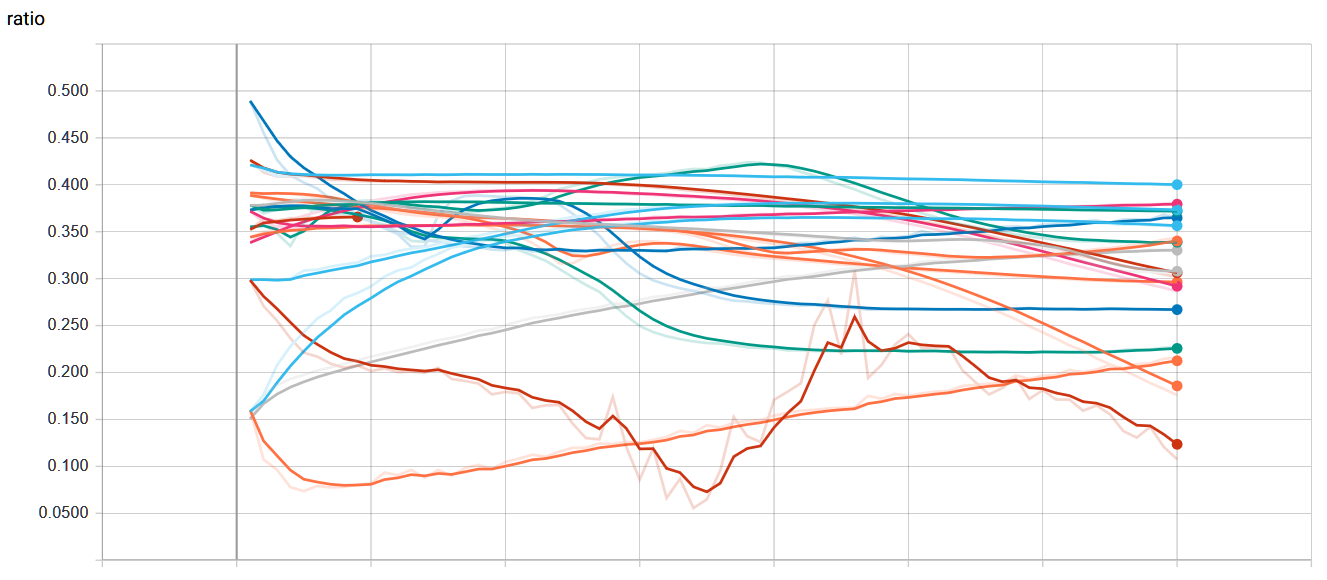
\includegraphics[width=0.7\textwidth]{images/sweep_35_ratio.png}
		\caption{\small The proportion of error not explained by a linear model of known invariants. Model demonstrated by the lowest red line achieved a ratio of  0.98 demonstrating nearly all of the variance was explained by known invariants. }
	\end{center}	
\end{figure}

These learned parameters served as a strong initial parameters for learning an invariant over trajectories of pendulum. This parameter-optimized model was trained to minimize the objective:
\begin{align}
\min_{\phi} \sum^{T}_{t = 1} &  
\left( \left\vert
\frac{\dot{\pmb{r}_t} \cdot \bigtriangledown \phi \left( \pmb{r}_t \right)}{{\Vert f_t \Vert}^2_2 * {\Vert \bigtriangledown \phi (\pmb{r}_t) \Vert}^2_2}
\right \vert
- \left( 1-\left\Vert \bigtriangledown \phi \left( \pmb{r}_t \right) \right\Vert^2_2 \right)^2 \right)
\end{align}
and the learned invariant displayed near zero variance along simulated trajectories while varying over the set of training trajectories. Figure 2 demonstrates the performance of the optimized model learning a non trivial function $\phi$ quickly and with near zero gradient along pendulum trajectories. During evaluation of this model, the sparse sampling of pendulum trajectories was identified to bias models, thus a faster RK4 differential equation solver was implemented to provide denser sampling pendulum trajectories.

\begin{figure}
\begin{center}
	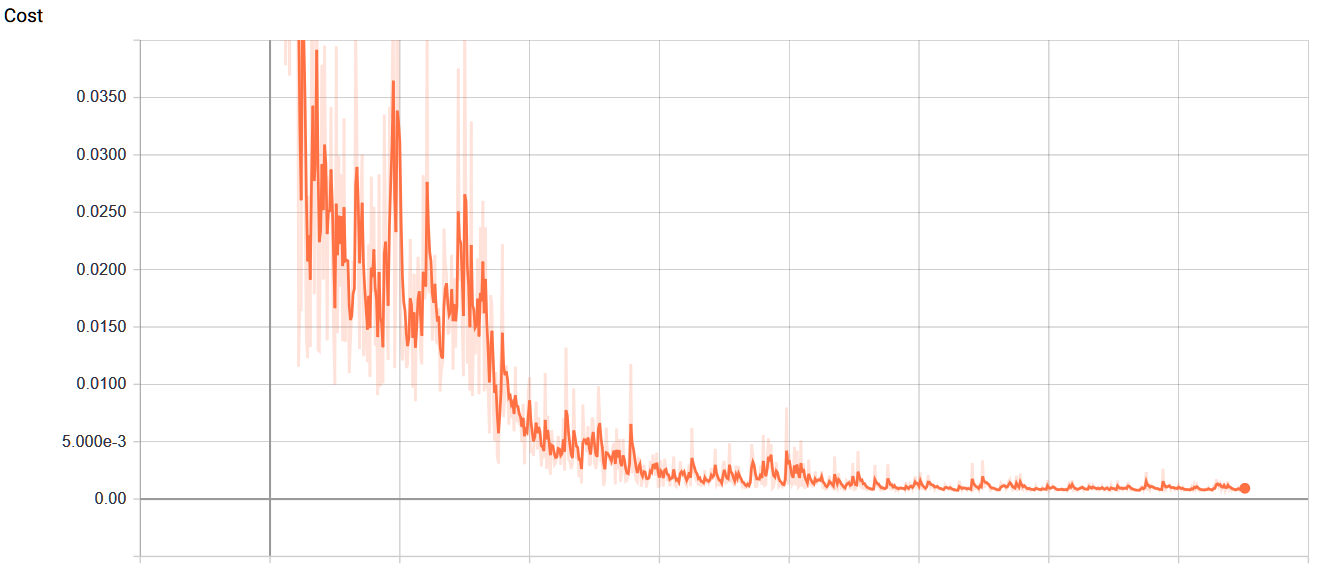
\includegraphics[width=0.49\textwidth]{images/pendulum_training.png}
	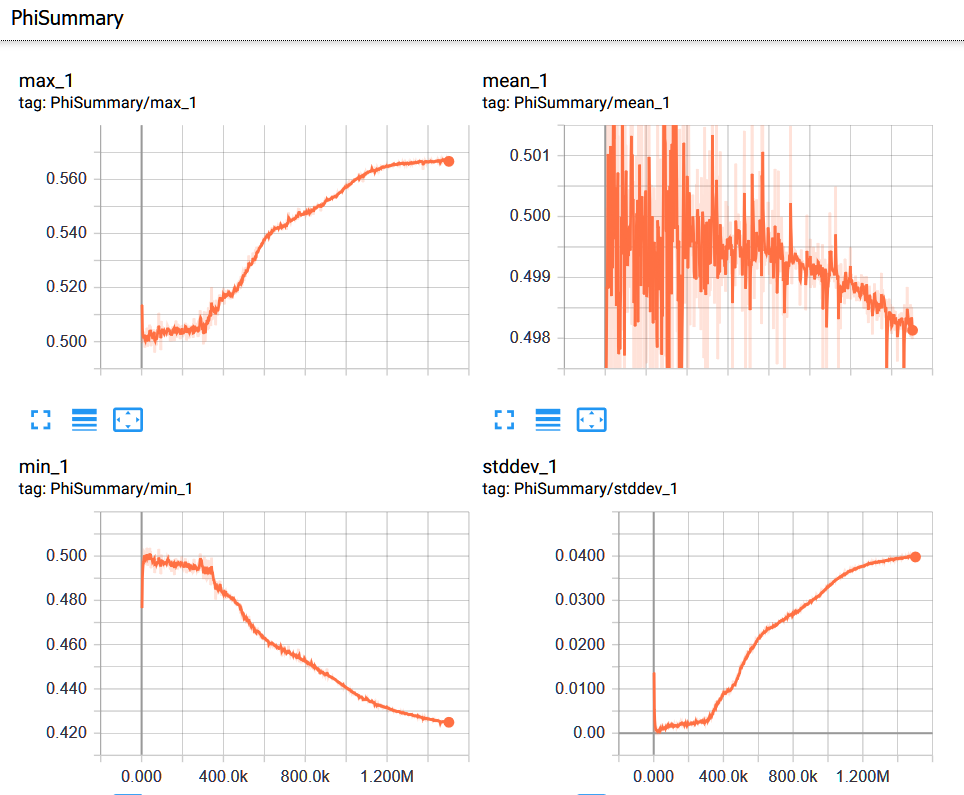
\includegraphics[width=0.49\textwidth]{images/Learned_phi_pendulum.png}
	\caption{\small (Left) $\dot{\pmb{r}_t} \cdot \bigtriangledown \phi \left( \pmb{r}_t \right)$ along test pendulum trajectories (Right) Summary statistics of learned invariant $\phi \left( \pmb{r}_t \right)$ over test set while training. Note the learned function is both non-trivial and constant along sampled trajectories  }
\end{center}	
\end{figure}

\begin{figure}
	\begin{center}
		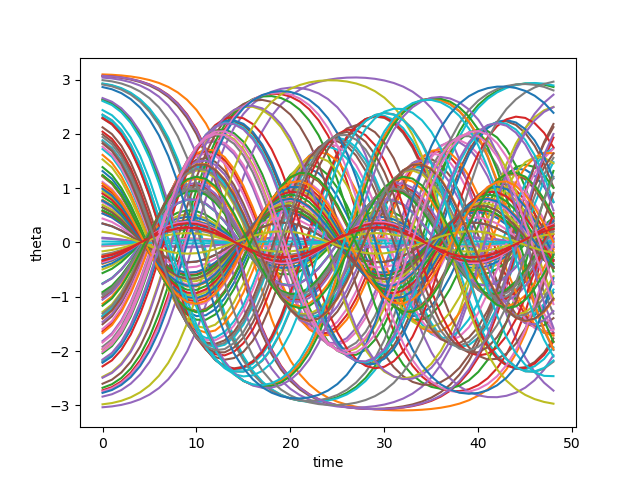
\includegraphics[width=0.49\textwidth]{images/Figure_1.png}
		\caption{\small Sampled pendulum trajectories simulated by RK4 solver}
	\end{center}	
\end{figure}


\end{document}